\scanpage{12}
% archive sheet number: 11
3) Supposons $\dot K\cap C=\emptyset$, et posons
\[
\begin{aligned}
 \unsure{\cdot|{}}B'&=U'_K\cap\dot K\\
 U'&=U'_K\setminus B'=\mathrm{Int}(U'_K)\\
 V'&=X\setminus\overline{U'_K}=(\underbrace{X\setminus U'_K}_{X'_1})\setminus C\\
   &=\mathrm{Int}(X'_1)
\end{aligned}
\]
\[
\deleted{U'=U'_K}
\]
enfin $W=V\cap V'=\complement K$.

\diagram{\begin{tikzcd}[ampersand replacement=\&,row sep=large,column sep=small]
 U^{\deleted{\unsure{'|1}}}\arrow[dr,no head,"B"'] \& \& U'\arrow[ll,"C"']\arrow[dl,no head,"B'"']\\
 \& W^{\deleted{\unsure{U|U\prime}}} \&
\end{tikzcd}}

\figure{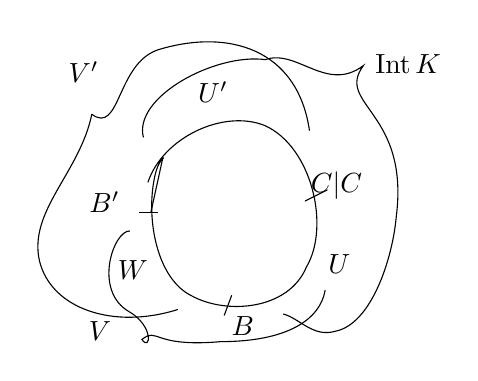
\begin{tikzpicture}[x=0.95cm,y=0.95cm]
\draw (0.88,3.06) .. controls (1.26,2.78) and (1.21,3.73) .. (1.76,3.92)
 .. controls (2.7,4.21) and (3.63,3.94) .. (3.79,2.84);
\draw (0.88,3.06) .. controls (0.72,2.28) and (0.03,1.77) .. (0.18,1.1)
 .. controls (0.34,0.45) and (1.18,0.18) .. (2.03,0.45);
\draw (1.57,2.75) .. controls (1.43,3.29) and (2.53,3.88) .. (3.20,3.79)
 .. controls (3.62,3.94) and (4.02,3.34) .. (4.51,3.71)
 .. controls (4.13,3.19) and (5.13,3.10) .. (4.95,1.69)
 .. controls (4.9,1.13) and (4.62,0.26) .. (4.14,0.16)
 .. controls (3.84,0.07) and (3.66,0.33) .. (3.44,0.39);
\draw (1.39,1.5) .. controls (1.17,1.51) and (0.89,0.70) .. (1.38,0.42)
 .. controls (1.72,0.22) and (1.66,-0.12) .. (1.55,0.05)
 .. controls (1.77,0.22) and (1.68,-0.06) .. (2.60,0.02)
 .. controls (3.47,0.02) and (3.93,0.30) .. (4.00,0.71);
\draw (1.63,2.15) .. controls (1.83,2.75) and (2.64,3.13) .. (3.19,2.91)
 .. controls (3.82,2.63) and (4.07,1.56) .. (3.75,1.02)
 .. controls (3.51,0.44) and (2.68,0.38) .. (2.22,0.63)
 .. controls (1.76,0.85) and (1.61,1.62) .. (1.71,2.17)
 .. controls (1.74,2.34) and (1.78,2.42) .. (1.84,2.48);
\draw (1.83,2.48)--(1.67,1.75);
\draw (1.51,1.75)--(1.76,1.75);
\draw (3.73,1.90)--(4.03,2.05);
\draw (2.75,0.64)--(2.65,0.37);
\node at (0.77,3.62) {$V'$}; \node at (2.50,3.36) {$U'$};
\node[right] at (4.54,3.73) {$\mathrm{Int}\,K$};
\node at (1.05,1.89) {$B'$}; \node at (4.15,2.11) {$\unsure{C|\mathbb C}$};
\node at (1.43,0.98) {$W$}; \node at (4.19,1.06) {$U$};
\node at (0.99,0.16) {$V$}; \node at (2.90,0.23) {$B$};
\end{tikzpicture}}

Alors on a :
\[
\begin{array}{ll|l}
 U,U',W&\text{ouverts disjoints}& U,U',W,B,B',C\\
 B,B',C&\text{fermés disjoints}&\text{pseudopartition de }X
\end{array}
\]
\[
\left\{\begin{aligned}
 &\overline U\cap\overline{U'}=C,\quad
 \overline U^{\deleted{\unsure{'|*}}}\cap\overline W=B,\quad
 \overline W\cap\overline{U'}=B'\\
 &\unsure{\dot U'|\overline{U'}}\deleted{\unsure{\setminus|{}}}=\overline{U'}\setminus U'=B'\cup C,\quad
 \dot U=B\cup C,\quad \dot W=B\cup B'\\
 &K=\overline{U\cup U'}=\complement W=(U\cup U')\cup B,\cup B'\cup C,\quad
 \mathrm{Int}\,K=(U\cup U'\cup C
\end{aligned}\right.
\]
\deleted{\illegible{1}}

4) \deleted{\unsure{Donnons|Posons}} Soient $U,U',W$ 3 ouverts d'un espace $X$.

Conditions équivalentes

a) $U,U',W$ mutuellement disjoints, réunion dense,
\[
 \overline U\cap\overline{U'}\cap\overline W=\emptyset,\quad
 \deleted{\unsure{\overline U|U}\unsure{\subset|\cap}}\dot U\subset\overline{U'\cup W},\quad
 \dot U'\subset\overline{U\deleted{\unsure{\cap|'}}\cup W},\quad
 \dot W\subset\overline{U\cup U'}
\]

b) Posant $C=\overline U\cap\overline{U'}$, $B=\overline U\cap\overline W$, $B'=\overline W\cap\overline{U'}$, les 6 ens $U,U',W,B,B',C$ forment une pseudopartition de $X$.

On a alors les relations ci-dessus --

Il revient au $=$ de se donner (pour $X$ fixe) $U,U',W$ satisfaisant les conditions \inserted{équ.} a) b), \unsure{ou|--} $K,$ \inserted{fermé de $X$} et $\underbrace{U_K,U'_K}_{\text{ouverts de }K}$ satisfaisant
\[
\left\{\begin{aligned}
 \overline{U_K}&=K\setminus U'_K,\quad \overline{W_K}=K\setminus U_K\\
 C\cap\dot K&=\emptyset\quad \text{(où}\quad C=\overline{U_K}\cap\overline{U'_K}=K\setminus(U_K\cup U'_K)
\end{aligned}\right.
\]
